\documentclass[a4paper,12pt]{article}
\usepackage{ctex}
\usepackage{geometry}
\geometry{a4paper, left=2.5cm, right=2.5cm, top=2.5cm, bottom=2.5cm}
\usepackage{amsmath, amssymb}
\usepackage{enumerate}
\usepackage{graphicx}
\usepackage{float}

\title{GEM Gaussian Embedding Modeling for Out of Distribution Detection in GUI Agents}
\author{Yang}

\begin{document}
\maketitle
\section{Introduction}
GUI Agent遇到的OOD问题:
\begin{itemize}
    \item Internalization OOD:在ID的环境中执行任务,但是错误的假设了存在不支持的功能(操作的APP在ID中,但是具体功能不在)
    \item Extrapolation OOD:工作于动态的不断演变的环境中,之前没见过(这个APP不在ID中)
\end{itemize}

GUI Agent的OOD问题可能会引发安全问题,因为模型处理OOD问题的能力依赖于泛化能力,可能会出错造成损失,因此检测OOD问题很重要

GUI Agent的OOD detection面临的问题:
\begin{itemize}
    \item Complex Embedding Space:屏幕包含的UI元素复杂度远高于MLLM且用户指令的多样性也更高
    \item Envolving Environment:系统的更新和新APP的出现会导致OOD检测需要不断迭代
\end{itemize}

\section{Challenges}
\subsection{Problem Formulation}
一个GUI Agent$F$首先经过$D_{ID}$的数据集的训练,然后给出user instruction$x$和屏幕截图$s$,之后根据这个输入,模型预测行为$a_t$并执行操作,直到完成任务或者超出最大步数限制。由此定义一个OOD检测函数:若$(s_t, x)$是OOD,则$f_{OOD}(s_t, x) = 1$

\subsection{Popular OOD Detection Method}
主要分类有两种:
\begin{itemize}
    \item Embedding-based:模型当下的ID存在一个embedding space(向量空间),可以将输入放入模型的向量空间比较分布之间的差距,用欧式距离等进行衡量
    \item Uncertainty-based:通常用熵、置信度等描述不确定性的量来衡量
\end{itemize}
其中Uncertainty-based效果更差,模型很难说明其不确定性,原因在于ID和OOD数据的可分性很低。

上述两种方法依赖于$Youden\space Index = arg\space max_{t}(TPR(t)-FPR(t))$,其中TPR与FPR分别代表true positive rate和false positive rate。而TP代表输入是ID,预测也是ID,FN代表输入是ID,预测是OOD,则$TPR = \frac{TP}{TP + FN}$.

而真正训练的数据集具有复杂性和多样性,但是他们的embedding space在距离上表现出明显的cluster(聚类)现象,即同一距离出现大量样本,不同聚类之间具有明显距离差距

\section{Algorithm}
首先定义encoder layer$l_e$,作用是将$(s_i, x_i)$映射到embedding vector,即$e_i = l_e(s_i, x_i)$,由此可以得到$D_{embedding}$。然后计算该数据集的centroid$\mu$,即$\mu = \frac{1}{k}\sum_{i=1}^{k}e_i$,然后计算Euclid distance,即$d_i = |e_i - \mu|_2$,得到$D_{distance}$。显然距离分布不是一个典型的分布,所以我们假设分布是由$m$个不同的高斯分布混合而成,那么有$p(d) = \sum_{j=1}^{m}\pi_jN(d|\mu_j, \sigma_j^2)$,且$\sum_{j=1}^{m}\pi_j = 1$,其中$N(d|\mu_j, \sigma_j^2)$代表该高斯分布概率密度函数代入$d$的取值。最后再计算log-likelihood:$logL_m = \sum_{i=1}^{k}p(d_i)$。该公式的参数包括$\{\pi_j, \mu_j, \sigma_j\}$,通过EM算法最大化log-likelihood得到。EM算法首先计算$\gamma_{ij} = \frac{\pi_jN(d_i|\mu_j, \sigma_j^2)}{p(d_i)}$,然后令$\pi_j^{new} = \frac{1}{k}\gamma_{ij}$,$\mu_j^{new} = \frac{\sum_{i=1}^{k}\gamma_{ij}d_i}{\sum_{i=1}^{k}\gamma_{ij}}$,$\sigma_j^{2 new} = \frac{\sum_{i=1}^{k}\gamma_{ij}(d_i - \mu_j^{new})^2}{\sum_{i=1}^{k}\gamma_{ij}}$,参数化$m$用BIC:$BIC(m) = -2logL_m + mlogk$。最后使用一个区间$[\mu_j - n\sigma_j, \mu_j + n\sigma_j]$,如果$d_i$落在某个区间里就认为不是OOD
\begin{figure}[H]
    \centering
    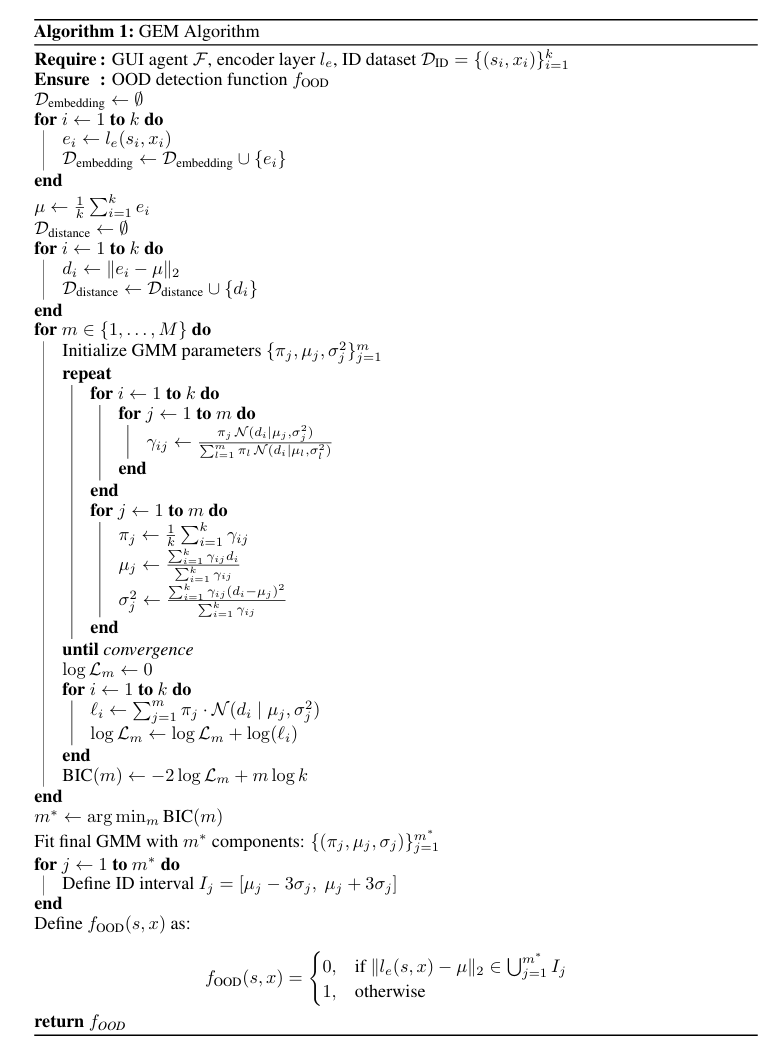
\includegraphics[width=\textwidth]{algorithm.png}
\end{figure}

\section{Result}
该方法很好的区分了ID与OOD,大部分准确率在95\%以上。除此之外研究神经网络检测层数和检测OOD准确率的情况,结果是开始随着层数加深而上升,之后开始下降,且有趣的是集中在第9层达到峰值(50\%的结果),因素有两个,一个是特殊任务相关的特征,另一个是视觉或文本的特征,在层数上升时,前者重要性增加,后者降低,在9层附近达到平衡

\section{Summary}
本篇论文讲述了一种应用于区分GUI Agent测试数据ID和OOD的方法,首先根据训练的数据绘制分布,然后在embedding空间里对测试数据进行向量化,应用混合高斯分布,利用算法求参数最优化结果,然后利用区间分布判断测试数据属于ID还是OOD,结果是显著提高了分辨的成功率
\end{document}